\chapter{Cplex}

CPLEX is a high-performance optimization software developed by IBM that specializes in solving mathematical programming problems, including linear programming, mixed-integer programming, and quadratic programming, among others. It is one of the most widely used commercial solvers for solving complex optimization problems in various industries and academic research.

CPLEX provides a comprehensive suite of algorithms and techniques to efficiently solve optimization problems of varying sizes and complexities. It employs state-of-the-art optimization algorithms, such as the primal-dual interior point method for linear programming and branch-and-bound algorithms for mixed-integer programming, to find high-quality solutions within reasonable timeframes. 

One of the key features of CPLEX is its ability to handle large-scale optimization problems efficiently. It incorporates advanced preprocessing techniques, presolve routines, and cutting-plane algorithms to reduce problem size and improve solution quality. Additionally, CPLEX offers parallel computing capabilities, leveraging multiple CPU cores and distributed computing environments to accelerate the solution process for large-scale problems.

Overall, CPLEX is a powerful optimization tool that enables users to model, solve, and analyze complex optimization problems across diverse domains, including operations research, logistics, supply chain management, finance, and engineering. Its robust performance, scalability, and versatility make it a valuable asset for researchers, practitioners, and organizations seeking to optimize their decision-making processes.

CPLEX is useful for solving the TSP due to its efficient solver, scalability for large instances, support for Mixed-Integer Programming formulations commonly used for TSP, integration with programming languages like Python, and parallel computing capabilities, enabling faster solution times for complex TSP instances.



\section{Integer Linear Programming Formulation of TSP}

In order to use CPLEX to solve the TSP we first need to define an integer linear programming (ILP) model for it. \\
Let's denote the graph as $G=(V,E)$, where $V$ represents the set of nodes (vertices) and $E$ represents the set of edges.
Let $n$ be the number of nodes in the graph, and let $c_{ij}$ represent the cost (weight) of traveling from node $i$ to node $j$ in the graph $G$. If there is no direct edge between nodes $i$ and $j$, we can set $c_{ij}$ to a large value to indicate that traveling between these nodes is not allowed. \\
A possbile ILP model can be formulated using the following decision variable
\begin{align*}
	& x_{ij} = 
	\begin{cases}
		1, & \text{if edge } (i,j)\in E \text{ is chosen in the optimal circuit}\\
		0, & \text{otherwise}
	\end{cases}
\end{align*}
Using fact that in a TSP solution each node has degree equal to two we obtain:
\begin{align}
	\text{min} &\sum\limits_{(i,j)\in E} c_{ij} \cdot x_{ij} \tag{1.1}\label{eq:1.1} \\
	&\sum\limits_{\:\;\;j=1\:\;\;}^{n} x_{ij} = 2 \quad \text{for } i = 1,2,\ldots,n \tag{1.2}\label{eq:1.2} \\
	&\sum\limits_{(i,j)\in C} x_{ij} \leq |C| - 1 \quad \forall \; C: C \text{ is a subtour of } G \tag{1.3}\label{eq:1.3}
\end{align}
where equation \eqref{eq:1.1} is the total cost of the circuit, constraints \eqref{eq:1.2} are the degree constraints and \eqref{eq:1.3} are the Subtour Elimination Constraints(SEC). Counting the number of constraints we have $n$ constraints from \eqref{eq:1.2} and an exponential amount from \eqref{eq:1.3}. A number of constraints that big makes in practice the problem much harder to resolve, so a common workaround also used in the following algorithms is to ignore SEC and add only the ones that are violated each time cplex returns a feasible solution.

\section{Initialization of CPLEX}

In order to use CPLEX we must initialize the problem first, that means write the TSP according to CPLEX standards. To do this we start with an empty problem and then proceed to add all necessary elements to represent the ILP formulation described previously.

To create the empty problem one must simply call the functions \textbf{CPXopenCPLEX} to initialize CPLEX itself and \textbf{CPXcreateprob} to create the empty problem.
Once the problem is created, it needs to be populated with variables (columns) and constratints (rows).
Variables denoted as $x_{ij}$ are added using function \textbf{CPXnewcols}.
This can be done either in a sequentially (one at a time) or all at the same time by allocating the necessary memory and passing all variables to CPLEX via arrays.
However this process can be tedious, with the exception of some cases in which it may be easier that way (for example if the data in the instance is saved in a similar way).
The next step involves adding constraints. As discussed earlier, it is more efficient to add only the constraints specified by Equation \eqref{eq:1.2} without any SEC constraints (\eqref{eq:1.3}).
The procedure for adding constraints is similar to that for variables: the function \textbf{CPXaddrows} can add multiple constraints at once or one at a time, similar to \textbf{CPXnewcols}.
Sequential addition tends to be more straightforward.
This procedure is summarized in the algorithm in \figurename{ \ref{fig:CPLEXinit}}.

\begin{figure}[htbp]
	\textbf{CPLEX Initialization} \\
	\begin{algorithm}[H]
		%\TitleOfAlgo{\textbf{CPLEX initialization}}
		\SetKwInOut{Input}{input}
		\SetKwInOut{Output}{output}
		\Input{Graph $G(V,E)$ fully connected \newline$c_{ij}=$ cost of $edge(i,j) \in |E|$ }
		\Output{Instance initialized in CPLEX}
		\vspace{2mm}
		Create empty CPLEX linear problem $p$\\
		\ForEach{edge $e_{ij} \in E$}{
			Add binary variable $x_{i,j}$ with associated cost $c_{ij}$ to $p$\\
		}
		\ForEach{$v \in \{1, \dots ,|V|\}$}{
			$s_v=\sum\limits_{(i,j) \in E} y_{ij}$ where $y_{ij} = 1 \iff i=v$ or $j=v$; otherwise $y_{i,j} = 0$\\
			Add constraint $s_v \leq 2$ to $p$\\
		}
		\Return{$p$}
	\end{algorithm}
	\caption{CPLEX initialization algorithm}\label{fig:CPLEXinit}
\end{figure}

\section{CPLEX edge representation}

This section describes the data format of the output of CPLEX as well as a different format that improves TSP specific algorithms.
When interacting with CPLEX the convention used for the solution is very important.
Since CPLEX solves the ILP formulation of the TSP any solution $x^*$ given as output is in the form of an array containing a binary variable $x_{ij}$ for each edge in $E$ as shown in \figurename{ \ref{fig:CPLEXxstar}}. 

\begin{figure}[htbp]
	\begin{center}
		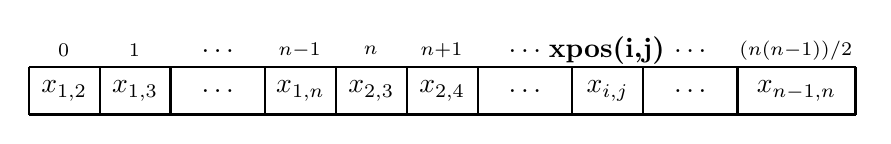
\begin{tikzpicture}[thick,scale=0.6]
			\draw (0,0) -- (17.5,0);
			\draw (0,1) -- (17.5,1);
			\foreach \p [count=\i from 0] in {0,1.5,3,5,6.5,8,9.5,11.5,13,15,17.5} {
				\draw (\p,0) -- (\p,1);
			}
			\path (.5,.5) (0.75,1.35) node{$_{0}$} ++(1.5,0) node{$_{1}$} ++(1.75,0) node{$\dots$} ++(1.75,0) 
									node{$_{n-1}$} ++(1.5,0) node{$_{n}$} ++(1.5,0) node{$_{n+1}$} ++(1.75,0) node{$\dots$} ++(1.75,0)
									node{$_{\textbf{xpos(i,j)}}$} ++(1.75,0) node{$\dots$} ++(2.25,0)
									node{$_{(n(n - 1)) / 2}$};
			\path (.5,.5) (0.75,0.5) node{$x_{1,2}$} ++(1.5,0) node{$x_{1,3}$} ++(1.75,0) node{$\dots$} ++(1.75,0) 
									node{$x_{1,n}$} ++(1.5,0) node{$x_{2,3}$} ++(1.5,0) node{$x_{2,4}$} ++(1.75,0) node{$\dots$} ++(1.75,0)
									node{$x_{i,j}$} ++(1.75,0) node{$\dots$} ++(2.25,0)
									node{$x_{n-1,n}$};
		\end{tikzpicture}
	\end{center}
	\caption{CPLEX solution array} \label{fig:CPLEXxstar}
\end{figure}

Given such an array it can be quite troublesome to find an edge given its connected nodes $(i,j)$.
To extract the position of edge $(i,j)$ one must use a function like the \textbf{xpos} function, as shown in \figurename{ \ref{fig:xpos}}.

\begin{figure}[htbp]
	\textbf{xpos} \\
	\begin{function}[H]
		%\TitleOfAlgo{\textbf{xpos}}
		\SetKwInOut{Input}{input}
		\SetKwInOut{Output}{output}
		\Input{$i$, $j$, $|V|$}
		\Output{position of $edge(i,j)$ in CPLEX notation}
		\vspace{2mm}
		\If{$i = j$}{ Error\; }
		\If{$i > j$}{ $i \Leftrightarrow j$\; }
		\Return{$i |V| + j - \frac{(i + 1) (i + 2)}{2}$}
	\end{function}
	\caption{xpos function}\label{fig:xpos}
\end{figure}

Saving the solution this way requires a lot of space as well as an increase in indexing complexity caused by the need use the \textbf{xpos} function.
Therefore, as soon as CPLEX is done, it's more efficient to convert the solution into a more specialized format.
The data structure used to store the solution in the previous chapters is not as straightforward to use.
This is because the output of CPLEX, as described in the following chapters, might contain two or more subtours.
Unfortunately, the solution format used until now cannot efficiently handle solutions containing subtours, necessitating the introduction of a different format.
The Successors format enables efficient storage of subtours without requiring additional structures or the use of the \textbf{xpos} function.
The format consists of an array of size $|V|$, where each position $i$ contains the index of the successor of node $i$ itself.
A comparison between all solution formats used in this project is illustrated in \figurename{ \ref{fig:cpxsuccEx}}.

\begin{figure}[htbp]
	\begin{center}
		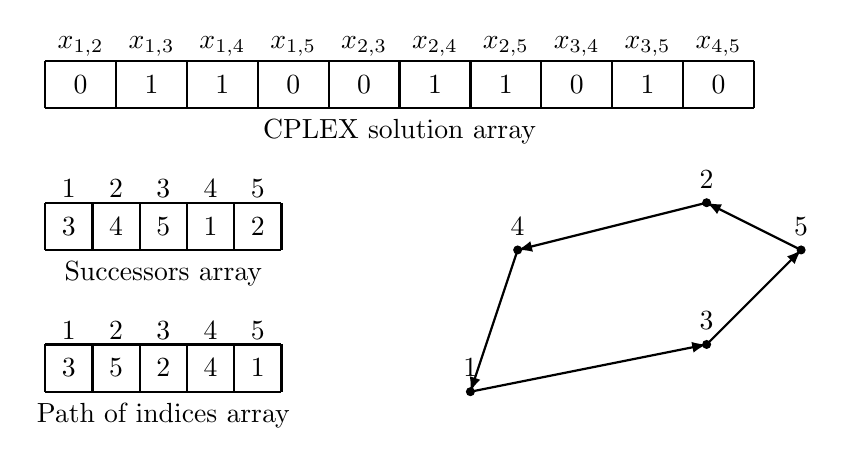
\begin{tikzpicture}[thick,scale=.6]
			% CPLEX ARRAY
			\path (.5,.5) (0.75,8.3) node{$x_{1,2}$} ++(1.5,0) node{$x_{1,3}$} ++(1.5,0) node{$x_{1,4}$} ++(1.5,0) node{$x_{1,5}$} ++(1.5,0)
									 node{$x_{2,3}$} ++(1.5,0) node{$x_{2,4}$} ++(1.5,0) node{$x_{2,5}$} ++(1.5,0) 
									 node{$x_{3,4}$} ++(1.5,0) node{$x_{3,5}$} ++(1.5,0)
									 node{$x_{4,5}$} ++(1.5,0);
			\path (.5,.5) (0.75,7.5) node{$0$} ++(1.5,0) node{$1$} ++(1.5,0) node{$1$} ++(1.5,0) node{$0$} ++(1.5,0)
									 node{$0$} ++(1.5,0) node{$1$} ++(1.5,0) node{$1$} ++(1.5,0) 
									 node{$0$} ++(1.5,0) node{$1$} ++(1.5,0)
									 node{$0$} ++(1.5,0);
			\draw (0,7) -- (15,7);
			\draw (0,8) -- (15,8);
			\foreach \p [count=\i from 0] in {0,1.5,3,4.5,6,7.5,9,10.5,12,13.5,15} {
				\draw (\p,7) -- (\p,8);
			}
			\draw (7.5,6.5) node{CPLEX solution array};
			
			% SUCCESSORS ARRAY
			\draw (0,4) grid (5,5);
			\draw (2.5,3.5) node{Successors array};
			\path (.5,.5) (0.5,5.3) node{$1$} ++(1,0) node{$2$} ++(1,0) node{$3$} ++(1,0) node{$4$} ++(1,0) node{$5$};
			\path (.5,.5) (0.5,4.5) node{$3$} ++(1,0) node{$4$} ++(1,0) node{$5$} ++(1,0) node{$1$} ++(1,0) node{$2$};

			% INDEXPATH ARRAY
			\draw (0,1) grid (5,2);
			\draw (2.5,0.5) node{Path of indices array};
			\path (.5,.5) (0.5,2.3) node{$1$} ++(1,0) node{$2$} ++(1,0) node{$3$} ++(1,0) node{$4$} ++(1,0) node{$5$};
			\path (.5,.5) (0.5,1.5) node{$3$} ++(1,0) node{$5$} ++(1,0) node{$2$} ++(1,0) node{$4$} ++(1,0) node{$1$};


			\foreach \p [count=\i] in {(9,1), (14,5), (14,2), (10,4), (16,4)} {
				\filldraw [black] \p circle (2pt);
				\draw \p+(0,0.5) node {\i};
			}
			\draw [-latex] (9,1) -- (14,2);
			\draw [-latex] (14,2) -- (16,4);
			\draw [-latex] (16,4) -- (14,5);
			\draw [-latex] (14,5) -- (10,4);
			\draw [-latex] (10,4) -- (9,1);
		\end{tikzpicture}
	\end{center}
	\caption{Cplex and Successors solution notations} \label{fig:cpxsuccEx}
\end{figure}
